\section{Weighted Interval Scheduling Problem}

\subsection*{The Problem}

Given an array of \emph{intervals} $A[1\cdots n]$, where $A[i] = (s(i),t(i))$ is an interval represented with
\emph{start-time} $s(i)$ and \emph{finish-time} $t(i)$, and value $v(i)$ associated with $A[i]$, we seek a \emph{compatible} subset $X\subset A$
such that the total value of the intervals in $X$, i.e., $\sum_{A[i]\in X} v(i)$,
is maximized. Again, $X$ is \emph{compatible} is defined as that intervals in $X$
are disjoint~(i.e., any two intervals in $X$ don't overlap).  See an instance in Figure~\ref{fig:interval}.
Clearly, this weighted interval scheduling problem is a generalization
of the interval scheduling problem introduced in last lecture,
for which each interval is associated with unit value, i.e., $v(i) = 1, 1\le i \le n$.


\begin{figure}[h]
\centering{

\tikzset{every picture/.style={line width=0.75pt}} %set default line width to 0.75pt        

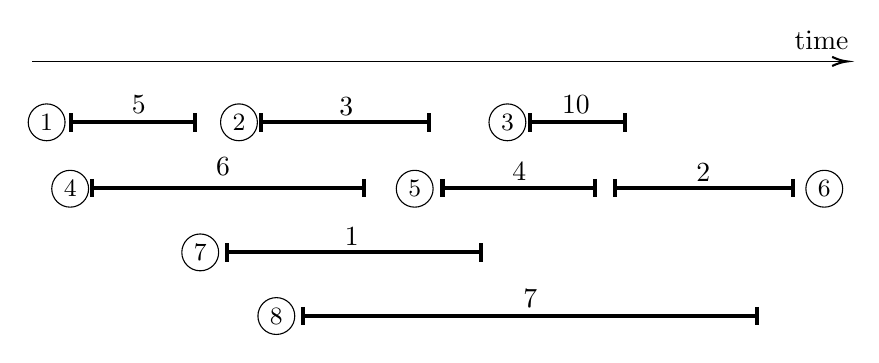
\begin{tikzpicture}[x=0.5pt,y=0.5pt,yscale=-1,xscale=1]
%uncomment if require: \path (0,248); %set diagram left start at 0, and has height of 248

%Straight Lines [id:da9015649955021968] 
\draw    (7,37) -- (594,37) ;
\draw [shift={(596,37)}, rotate = 180] [color={rgb, 255:red, 0; green, 0; blue, 0 }  ][line width=0.75]    (10.93,-3.29) .. controls (6.95,-1.4) and (3.31,-0.3) .. (0,0) .. controls (3.31,0.3) and (6.95,1.4) .. (10.93,3.29)   ;
%Straight Lines [id:da9640237890291299] 
\draw [line width=1.5]    (35,81) -- (124.5,81) ;
\draw [shift={(124.5,81)}, rotate = 180] [color={rgb, 255:red, 0; green, 0; blue, 0 }  ][line width=1.5]    (0,6.71) -- (0,-6.71)   ;
\draw [shift={(35,81)}, rotate = 180] [color={rgb, 255:red, 0; green, 0; blue, 0 }  ][line width=1.5]    (0,6.71) -- (0,-6.71)   ;
%Straight Lines [id:da3355888679808179] 
\draw [line width=1.5]    (172,81) -- (293.5,81) ;
\draw [shift={(293.5,81)}, rotate = 180] [color={rgb, 255:red, 0; green, 0; blue, 0 }  ][line width=1.5]    (0,6.71) -- (0,-6.71)   ;
\draw [shift={(172,81)}, rotate = 180] [color={rgb, 255:red, 0; green, 0; blue, 0 }  ][line width=1.5]    (0,6.71) -- (0,-6.71)   ;
%Straight Lines [id:da09988799250468405] 
\draw [line width=1.5]    (367,81) -- (435.5,81) ;
\draw [shift={(435.5,81)}, rotate = 180] [color={rgb, 255:red, 0; green, 0; blue, 0 }  ][line width=1.5]    (0,6.71) -- (0,-6.71)   ;
\draw [shift={(367,81)}, rotate = 180] [color={rgb, 255:red, 0; green, 0; blue, 0 }  ][line width=1.5]    (0,6.71) -- (0,-6.71)   ;
%Straight Lines [id:da4026459071674142] 
\draw [line width=1.5]    (50,128.5) -- (246.5,128.5) ;
\draw [shift={(246.5,128.5)}, rotate = 180] [color={rgb, 255:red, 0; green, 0; blue, 0 }  ][line width=1.5]    (0,6.71) -- (0,-6.71)   ;
\draw [shift={(50,128.5)}, rotate = 180] [color={rgb, 255:red, 0; green, 0; blue, 0 }  ][line width=1.5]    (0,6.71) -- (0,-6.71)   ;
%Straight Lines [id:da5509115882034084] 
\draw [line width=1.5]    (303.5,128.5) -- (413.5,128.5) ;
\draw [shift={(413.5,128.5)}, rotate = 180] [color={rgb, 255:red, 0; green, 0; blue, 0 }  ][line width=1.5]    (0,6.71) -- (0,-6.71)   ;
\draw [shift={(303.5,128.5)}, rotate = 180] [color={rgb, 255:red, 0; green, 0; blue, 0 }  ][line width=1.5]    (0,6.71) -- (0,-6.71)   ;
%Straight Lines [id:da6271509388583772] 
\draw [line width=1.5]    (428,128.5) -- (556.5,128.5) ;
\draw [shift={(556.5,128.5)}, rotate = 180] [color={rgb, 255:red, 0; green, 0; blue, 0 }  ][line width=1.5]    (0,6.71) -- (0,-6.71)   ;
\draw [shift={(428,128.5)}, rotate = 180] [color={rgb, 255:red, 0; green, 0; blue, 0 }  ][line width=1.5]    (0,6.71) -- (0,-6.71)   ;
%Straight Lines [id:da26802882985941956] 
\draw [line width=1.5]    (147.5,175) -- (331,175) ;
\draw [shift={(331,175)}, rotate = 180] [color={rgb, 255:red, 0; green, 0; blue, 0 }  ][line width=1.5]    (0,6.71) -- (0,-6.71)   ;
\draw [shift={(147.5,175)}, rotate = 180] [color={rgb, 255:red, 0; green, 0; blue, 0 }  ][line width=1.5]    (0,6.71) -- (0,-6.71)   ;
%Straight Lines [id:da22029647624095072] 
\draw [line width=1.5]    (202.5,221) -- (531,221) ;
\draw [shift={(531,221)}, rotate = 180] [color={rgb, 255:red, 0; green, 0; blue, 0 }  ][line width=1.5]    (0,6.71) -- (0,-6.71)   ;
\draw [shift={(202.5,221)}, rotate = 180] [color={rgb, 255:red, 0; green, 0; blue, 0 }  ][line width=1.5]    (0,6.71) -- (0,-6.71)   ;

% Text Node
\draw (556,13) node [anchor=north west][inner sep=0.75pt]   [align=left] {time};
% Text Node
\draw    (17.38, 81) circle [x radius= 13.31, y radius= 13.31]   ;
\draw (17.38,81) node  [font=\small] [align=left] {$\displaystyle 1$};
% Text Node
\draw    (156.38, 81) circle [x radius= 13.31, y radius= 13.31]   ;
\draw (156.38,81) node  [font=\small] [align=left] {$\displaystyle 2$};
% Text Node
\draw    (350.38, 81) circle [x radius= 13.31, y radius= 13.31]   ;
\draw (350.38,81) node  [font=\small] [align=left] {$\displaystyle 3$};
% Text Node
\draw    (34.38, 129) circle [x radius= 13.31, y radius= 13.31]   ;
\draw (34.38,129) node  [font=\small] [align=left] {$\displaystyle 4$};
% Text Node
\draw    (283.38, 129) circle [x radius= 13.31, y radius= 13.31]   ;
\draw (283.38,129) node  [font=\small] [align=left] {$\displaystyle 5$};
% Text Node
\draw    (579.38, 129) circle [x radius= 13.31, y radius= 13.31]   ;
\draw (579.38,129) node  [font=\small] [align=left] {$\displaystyle 6$};
% Text Node
\draw    (128.38, 175) circle [x radius= 13.31, y radius= 13.31]   ;
\draw (128.38,175) node  [font=\small] [align=left] {$\displaystyle 7$};
% Text Node
\draw    (183.38, 221) circle [x radius= 13.31, y radius= 13.31]   ;
\draw (183.38,221) node  [font=\small] [align=left] {$\displaystyle 8$};
% Text Node
\draw (77,60) node [anchor=north west][inner sep=0.75pt]   [align=left] {$\displaystyle 5$};
% Text Node
\draw (227,61) node [anchor=north west][inner sep=0.75pt]   [align=left] {$\displaystyle 3$};
% Text Node
\draw (388,60) node [anchor=north west][inner sep=0.75pt]   [align=left] {$\displaystyle 10$};
% Text Node
\draw (138,105) node [anchor=north west][inner sep=0.75pt]   [align=left] {$\displaystyle 6$};
% Text Node
\draw (352,108) node [anchor=north west][inner sep=0.75pt]   [align=left] {$\displaystyle 4$};
% Text Node
\draw (485,109) node [anchor=north west][inner sep=0.75pt]   [align=left] {$\displaystyle 2$};
% Text Node
\draw (231,155) node [anchor=north west][inner sep=0.75pt]   [align=left] {$\displaystyle 1$};
% Text Node
\draw (360,200) node [anchor=north west][inner sep=0.75pt]   [align=left] {$\displaystyle 7$};


\end{tikzpicture}

}
\caption{An instance of the weighted interval scheduling problem.
The optimal solution includes 3 intervals $\{1, 2, 3\}$,
and the (optimal) total value is 18.}
\label{fig:interval}
\end{figure}

Can we also design a greedy algorithm like we did for the interval scheduling problem?
Let's try. Again the framework is to maintain a compatible subset $X$, and
in each iteration we add one more interval that is compatible with $X$.
We now explore different greedy strategies. 

\vspace*{-\topsep}
\begin{enumerate}
\item In each iteration, pick the interval with the earliest finish-time that is compatible with $X$---which has been proved optimal for the unit-value version.
However, this strategy isn't optimal here---Figure~\ref{fig:interval} is an counter-example, where this greedy strategy finds intervals $\{1, 2, 5, 6\}$ with a total value of 14.
\item In each iteration, pick the interval with largest value that is compatible with $X$.
This strategy isn't optimal either.
Figure~\ref{fig:interval} is again a counter-example, where this greedy strategy finds intervals $\{3, 4\}$ with a total value of 16.
\end{enumerate}

As you can see, all these greedy strategies fail. In fact, it's unlikely to design a greedy algorithm for this problem.
We therefore seek other techniques. Below we will design a dynamic programming algorithm.

\subsection*{A Dynamic Programming Algorithm}

Recall that in order to design a DP algorithm, we need to figure out its \emph{optimal substructure}.
Does this problem satisfy the optimal substructure property?
Let's check Figure~\ref{fig:interval} to try to get some clue.
In that example, the \emph{optimal solution} is a set of intervals, namely $X = \{A[1], A[2], A[3]\}$.
Naturally, the \emph{substructure} of this optimal solustion is one of its subset, say, $X' = \{A[1], A[2]\}$, by removing one element $A[3]$.
Then we ask: is $X'$ the \emph{optimal solution} of certain subproblem?
In fact, yes! If we exclude $A[3]$ and all intervals that conflict with $A[3]$ from $A$,
the remaining will be $A' = \{A[1], A[2], A[4], A[7]\}$, and $X'$ is 
the \emph{optimal solution} of $A'$. (The proof is again a replacing argument: if there exists a
better solution~(than $X'$) of $A'$, then we can combine it with $A[3]$ to get a better solution of $A$.)
So, this problem indeed satisfies an optimal substructure property, and therefore a DP algorithm can be designed.

In fact, a direct use of above optimal substructure leads to exponential number of subproblems~(as we need to
define a subproblem for \emph{every} possible subset of $A$). We need an ordering to reduce
the number of subproblems.  Again, we can sort all intervals by their finish-time~(and rename them;
now we assume that all intervals in $A$ are sorted; see Figure~\ref{fig:order}).
Now let's check the optimal substructure again with sorted intervals.
The optimal solution is $X = \{A[1], A[3], A[6]\}$.
Consider its substructure $X' = \{A[1], A[3]\}$ by removing the last one in the order, i.e., $A[6]$.
We have that $X'$ is the optimal solution of $A[1\cdots 4]$. (Again, try the replacement-argument to prove it).
And why $A[1\cdots 4]$? This is because these four intervals do not overlap with $A[6]$ but $A[5]$ does.
In other words, $A[4]$ is the \emph{rightmost interval before $A[6]$ that doesn't conflict with $A[6]$}.
In fact, if $A[4]$ don't overlap with $A[6]$, i.e, $t(4)\le s(6)$, then all intervals to the left of $A[4]$ will not overlap with $A[6]$
as $t(1) \le t(2) \le t(3) \le t(4)$. 

\begin{figure}[h]
\centering{

\tikzset{every picture/.style={line width=0.75pt}} %set default line width to 0.75pt        

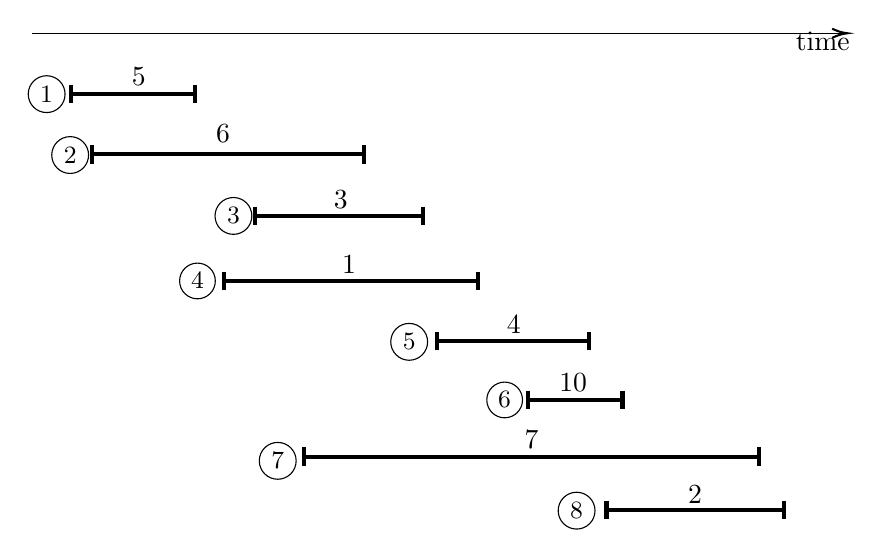
\begin{tikzpicture}[x=0.5pt,y=0.5pt,yscale=-1,xscale=1]
%uncomment if require: \path (0,383); %set diagram left start at 0, and has height of 383

%Straight Lines [id:da9015649955021968] 
\draw    (5,13) -- (592,13) ;
\draw [shift={(594,13)}, rotate = 180] [color={rgb, 255:red, 0; green, 0; blue, 0 }  ][line width=0.75]    (10.93,-3.29) .. controls (6.95,-1.4) and (3.31,-0.3) .. (0,0) .. controls (3.31,0.3) and (6.95,1.4) .. (10.93,3.29)   ;
%Straight Lines [id:da9640237890291299] 
\draw [line width=1.5]    (33,57) -- (122.5,57) ;
\draw [shift={(122.5,57)}, rotate = 180] [color={rgb, 255:red, 0; green, 0; blue, 0 }  ][line width=1.5]    (0,6.71) -- (0,-6.71)   ;
\draw [shift={(33,57)}, rotate = 180] [color={rgb, 255:red, 0; green, 0; blue, 0 }  ][line width=1.5]    (0,6.71) -- (0,-6.71)   ;
%Straight Lines [id:da3355888679808179] 
\draw [line width=1.5]    (166,145) -- (287.5,145) ;
\draw [shift={(287.5,145)}, rotate = 180] [color={rgb, 255:red, 0; green, 0; blue, 0 }  ][line width=1.5]    (0,6.71) -- (0,-6.71)   ;
\draw [shift={(166,145)}, rotate = 180] [color={rgb, 255:red, 0; green, 0; blue, 0 }  ][line width=1.5]    (0,6.71) -- (0,-6.71)   ;
%Straight Lines [id:da09988799250468405] 
\draw [line width=1.5]    (363,278) -- (431.5,278) ;
\draw [shift={(431.5,278)}, rotate = 180] [color={rgb, 255:red, 0; green, 0; blue, 0 }  ][line width=1.5]    (0,6.71) -- (0,-6.71)   ;
\draw [shift={(363,278)}, rotate = 180] [color={rgb, 255:red, 0; green, 0; blue, 0 }  ][line width=1.5]    (0,6.71) -- (0,-6.71)   ;
%Straight Lines [id:da4026459071674142] 
\draw [line width=1.5]    (48,100.5) -- (244.5,100.5) ;
\draw [shift={(244.5,100.5)}, rotate = 180] [color={rgb, 255:red, 0; green, 0; blue, 0 }  ][line width=1.5]    (0,6.71) -- (0,-6.71)   ;
\draw [shift={(48,100.5)}, rotate = 180] [color={rgb, 255:red, 0; green, 0; blue, 0 }  ][line width=1.5]    (0,6.71) -- (0,-6.71)   ;
%Straight Lines [id:da5509115882034084] 
\draw [line width=1.5]    (297.5,235.5) -- (407.5,235.5) ;
\draw [shift={(407.5,235.5)}, rotate = 180] [color={rgb, 255:red, 0; green, 0; blue, 0 }  ][line width=1.5]    (0,6.71) -- (0,-6.71)   ;
\draw [shift={(297.5,235.5)}, rotate = 180] [color={rgb, 255:red, 0; green, 0; blue, 0 }  ][line width=1.5]    (0,6.71) -- (0,-6.71)   ;
%Straight Lines [id:da6271509388583772] 
\draw [line width=1.5]    (420,357.5) -- (548.5,357.5) ;
\draw [shift={(548.5,357.5)}, rotate = 180] [color={rgb, 255:red, 0; green, 0; blue, 0 }  ][line width=1.5]    (0,6.71) -- (0,-6.71)   ;
\draw [shift={(420,357.5)}, rotate = 180] [color={rgb, 255:red, 0; green, 0; blue, 0 }  ][line width=1.5]    (0,6.71) -- (0,-6.71)   ;
%Straight Lines [id:da26802882985941956] 
\draw [line width=1.5]    (143.5,192) -- (327,192) ;
\draw [shift={(327,192)}, rotate = 180] [color={rgb, 255:red, 0; green, 0; blue, 0 }  ][line width=1.5]    (0,6.71) -- (0,-6.71)   ;
\draw [shift={(143.5,192)}, rotate = 180] [color={rgb, 255:red, 0; green, 0; blue, 0 }  ][line width=1.5]    (0,6.71) -- (0,-6.71)   ;
%Straight Lines [id:da22029647624095072] 
\draw [line width=1.5]    (201.5,319) -- (530,319) ;
\draw [shift={(530,319)}, rotate = 180] [color={rgb, 255:red, 0; green, 0; blue, 0 }  ][line width=1.5]    (0,6.71) -- (0,-6.71)   ;
\draw [shift={(201.5,319)}, rotate = 180] [color={rgb, 255:red, 0; green, 0; blue, 0 }  ][line width=1.5]    (0,6.71) -- (0,-6.71)   ;

% Text Node
\draw (555,10) node [anchor=north west][inner sep=0.75pt]   [align=left] {time};
% Text Node
\draw    (15.38, 57) circle [x radius= 13.31, y radius= 13.31]   ;
\draw (15.38,57) node  [font=\small] [align=left] {$\displaystyle 1$};
% Text Node
\draw    (150.38, 145) circle [x radius= 13.31, y radius= 13.31]   ;
\draw (150.38,145) node  [font=\small] [align=left] {$\displaystyle 3$};
% Text Node
\draw    (346.38, 278) circle [x radius= 12.9, y radius= 12.9]   ;
\draw (346.38,278) node  [font=\small] [align=left] {6};
% Text Node
\draw    (32.38, 101) circle [x radius= 13.31, y radius= 13.31]   ;
\draw (32.38,101) node  [font=\small] [align=left] {$\displaystyle 2$};
% Text Node
\draw    (277.38, 236) circle [x radius= 13.31, y radius= 13.31]   ;
\draw (277.38,236) node  [font=\small] [align=left] {$\displaystyle 5$};
% Text Node
\draw    (398.38, 358) circle [x radius= 13.31, y radius= 13.31]   ;
\draw (398.38,358) node  [font=\small] [align=left] {$\displaystyle 8$};
% Text Node
\draw    (124.38, 192) circle [x radius= 12.9, y radius= 12.9]   ;
\draw (124.38,192) node  [font=\small] [align=left] {4};
% Text Node
\draw    (182.38, 322) circle [x radius= 13.31, y radius= 13.31]   ;
\draw (182.38,322) node  [font=\small] [align=left] {$\displaystyle 7$};
% Text Node
\draw (75,36) node [anchor=north west][inner sep=0.75pt]   [align=left] {$\displaystyle 5$};
% Text Node
\draw (221,125) node [anchor=north west][inner sep=0.75pt]   [align=left] {$\displaystyle 3$};
% Text Node
\draw (384,257) node [anchor=north west][inner sep=0.75pt]   [align=left] {$\displaystyle 10$};
% Text Node
\draw (136,77) node [anchor=north west][inner sep=0.75pt]   [align=left] {$\displaystyle 6$};
% Text Node
\draw (346,215) node [anchor=north west][inner sep=0.75pt]   [align=left] {$\displaystyle 4$};
% Text Node
\draw (477,338) node [anchor=north west][inner sep=0.75pt]   [align=left] {$\displaystyle 2$};
% Text Node
\draw (227,172) node [anchor=north west][inner sep=0.75pt]   [align=left] {$\displaystyle 1$};
% Text Node
\draw (359,298) node [anchor=north west][inner sep=0.75pt]   [align=left] {$\displaystyle 7$};


\end{tikzpicture}

}
\caption{An instance of the weighted interval scheduling problem.
The optimal solution includes 3 intervals $\{1, 2, 3\}$,
and the (optimal) total value is 18.}
\label{fig:order}
\end{figure}


Above analysis suggests we define subproblem over $A[1\cdots k]$ for every $1\le k \le n$.
Formally, we define $F(k)$ be the achievable total value over the first $k$ intervals, i.e., $A[1\cdots k]$.
We now develop a recursion. Again, we try to enumerate all possiblities of the last step.
Here, that's whether $A[k]$ is picked or not. Suppose that, the optimal solution~(of $A[1\cdots k]$)
doesn't include $A[k]$; in this case we have $F(k) = F(k-1)$.
Suppose that, the optimal solution includes $A[k]$; in this case we have $F(k) = v(k) + F(pre[k])$.
Here, we use term $pre[k]$ to represent the \emph{rightmost interval before $A[k]$ that doesn't conflict with $A[k]$}.
Formally, $pre[k] = \max\{j < k \mid t(j) \le s(k)\}$.
Combined, we have the following recursion.

\begin{displaymath}
F(k) = \max\left\{
	\begin{array}{lll}
		F(k-1) \\
		F(pre[k]) + v(k)
	\end{array}
\right.
\end{displaymath}

One question remain: how to calculate $pre[k]$? One straitforward approach is to 
compare $A[k]$ with all intervals before $A[k]$ in reverse order, i.e., $A[k-1], A[k-2], \cdots, A[1]$;
the first $A[j]$ satisfies that $t(j) \le s(k)$ will be $pre[k]$. 
This clearly takes linear time. In fact, we can use \emph{binary search} to get a $O(\log n)$-time algorithm.
This works because, all intervals in $A$ are already sorted by their finish-time.

Specifically, we define a recursive function \emph{binary-search~($A[1\cdots n]$, $k$, $a$, $b$)}
with 4 parameters: $A[1\cdots n]$ is the sorted $n$ intervals, $k$ specifies that we aim to calculate $pre[k]$,
$a$ and $b$ specifies the range of $A$ where we will search for. 
%Formally, we define this recursive function returns $\max\{a \le j \le b \mid t(j) \le s(k)\}$. 
Its pseudo-code is given below.
Clearly, this binary-search procedure runs in $O(\log n)$ time.
To find $pre[k]$, we actually call: \emph{binary-search~($A$, $k$, $1$, $k-1$)}.

\begin{minipage}{0.8\textwidth}
	\aaA {11}{function binary-search~($A[1\cdots n]$, $k$, $a$, $b$)}\xxx
	\aab {$m = (a + b) / 2$;}\xxx
	\aaB {2}{if~($t(m) \le s(k) \le t(m + 1)$)\ \ // $pre[k] = m$}\xxx
	\aac {return $m$;}\xxx
	\aaB {2}{else if~($t(m) > s(k)$)\ \ // $pre[k]$ must be in $[a\cdots m]$}\xxx
	\aac {return binary-search~($A$, $k$, $a$, $m$);}\xxx
	\aaB {2}{else if~($s(k) > t(m + 1)$) \ \ // $pre[k]$ must be in $[m + 1\cdots b]$}\xxx
	\aac {return binary-search~($A$, $k$, $m + 1$, $b$);}\xxx
	\aaB {2}{else}\xxx
	\aac {return 0;}\xxx
	\aab {end;}\xxx
	\aaa {end;}\xxx
\end{minipage}

The complete DP algorithm for solving the weighted interval scheduling problem is given below.
Its running time is $O(n\log n)$: the sorting step takes $\Theta(n\log n)$, and for each $k$,
the binary-search takes $O(\log n)$, and hence the entire for-loop takes $O(n\log n)$ as
well.

\begin{minipage}{0.8\textwidth}
	\aaA {8}{Algorithm DP-weighted~(intervals $A[1\cdots n]$, $v(i)$, $1\le i \le n$)}\xxx
	\aab {sort $A$ by their finish-time;}\xxx
	\aab {init array $F$ of size $n + 1$ and set $F[0] = 0$;}\xxx
	\aaB {3}{for $k = 1 \to n$}\xxx
	\aac {$pre[k]$ = binary-search~($A$, $k$, $1$, $k-1$);}\xxx
	\aac {$F[k] = \max\{F[k-1], F[pre[k]] + v(k)\}$;}\xxx
	\aab {end;}\xxx
	\aab {return $F[n]$;}\xxx
	\aaa {end;}\xxx
\end{minipage}

